%
% Modified by Megan Patnott
% Last Change: Jan 18, 2013
%
%%%%%%%%%%%%%%%%%%%%%%%%%%%%%%%%%%%%%%%%%%%%%%%%%%%%%%%%%%%%%%%%%%%%%%%%
%
% Modified by Sameer Vijay
% Last Change: Tue Jul 26 2005 13:00 CEST
%
%%%%%%%%%%%%%%%%%%%%%%%%%%%%%%%%%%%%%%%%%%%%%%%%%%%%%%%%%%%%%%%%%%%%%%%%
%
% Sample Notre Dame Thesis/Dissertation
% Using Donald Peterson's ndthesis classfile
%
% Written by Jeff Squyres and Don Peterson
%
% Provided by the Information Technology Committee of
%   the Graduate Student Union
%   http://www.gsu.nd.edu/
%
% Nothing in this document is serious except the format.  :-)
%
% If you have any suggestions, comments, questions, please send e-mail
% to: ndthesis@gsu.nd.edu
%
%%%%%%%%%%%%%%%%%%%%%%%%%%%%%%%%%%%%%%%%%%%%%%%%%%%%%%%%%%%%%%%%%%%%%%%%


%
% Chapter 2
%

\chapter{Experimental Setup}

\section{Overview}

To measure conversion electrons for nuclear structure, three separate experiments were performed at the Nuclear Science Laboratory (NSL) at the University of the Notre Dame using the Internal Conversion Electron Ball (ICEBall) Spectrometer paired with several configurations of High Purity Germanium (HPGe) detectors. A Sm$(\alpha,2n)$Ge reaction was used with different enriched targets to create the desired Gd isotope.

\section{Nuclear Science Laboratory at Notre Dame}

The Nuclear Science Laboratory at the University of Notre Dame has been in operation since the 1930s. Currently, the NSL operates with three accelerators: the 10 MV FN Tandem, the 5 MV Sta. Ana accelerator, and the 3 MV 9S Tandem. The experiments in this dissertation were performed on the 10 MV FN Tandem.

The FN Tandem has two ion sources: the Helium Ion Source (HIS) and the Multi-Cathode Source of Negative Ions Using Cesium Sputtering (MC-SNICS). Most elements can take the electrons from Cesium to create negative ions. Helium, however, cannot, and needs a special source, as discussed below. For the experiments described, the HIS was used.

Due to the electron binding energy of Helium The HIS uses a duoplasmatron. Within the duoplasmatron, a thin tungsten wire is heated while surrounded by the source gas (Helium). The tungsten wire emits electrons, and positively ionizes the Helium. This helium is extracted from the duoplasmatron and focused by an einzel lens, where it then goes through the Lithium Charge Exchange. This section of the HIS works much like the Tandem, although the charge exchange works in reverse. The positively charged ions are accelerated through a Lithium vapor, and some gain electrons, becoming neutral or negatively charged. Those ions that become negatively charged are accelerated out the other end of the duoplasmatron, before being sent to the FN Tandem.

\begin{figure}
    \centering
    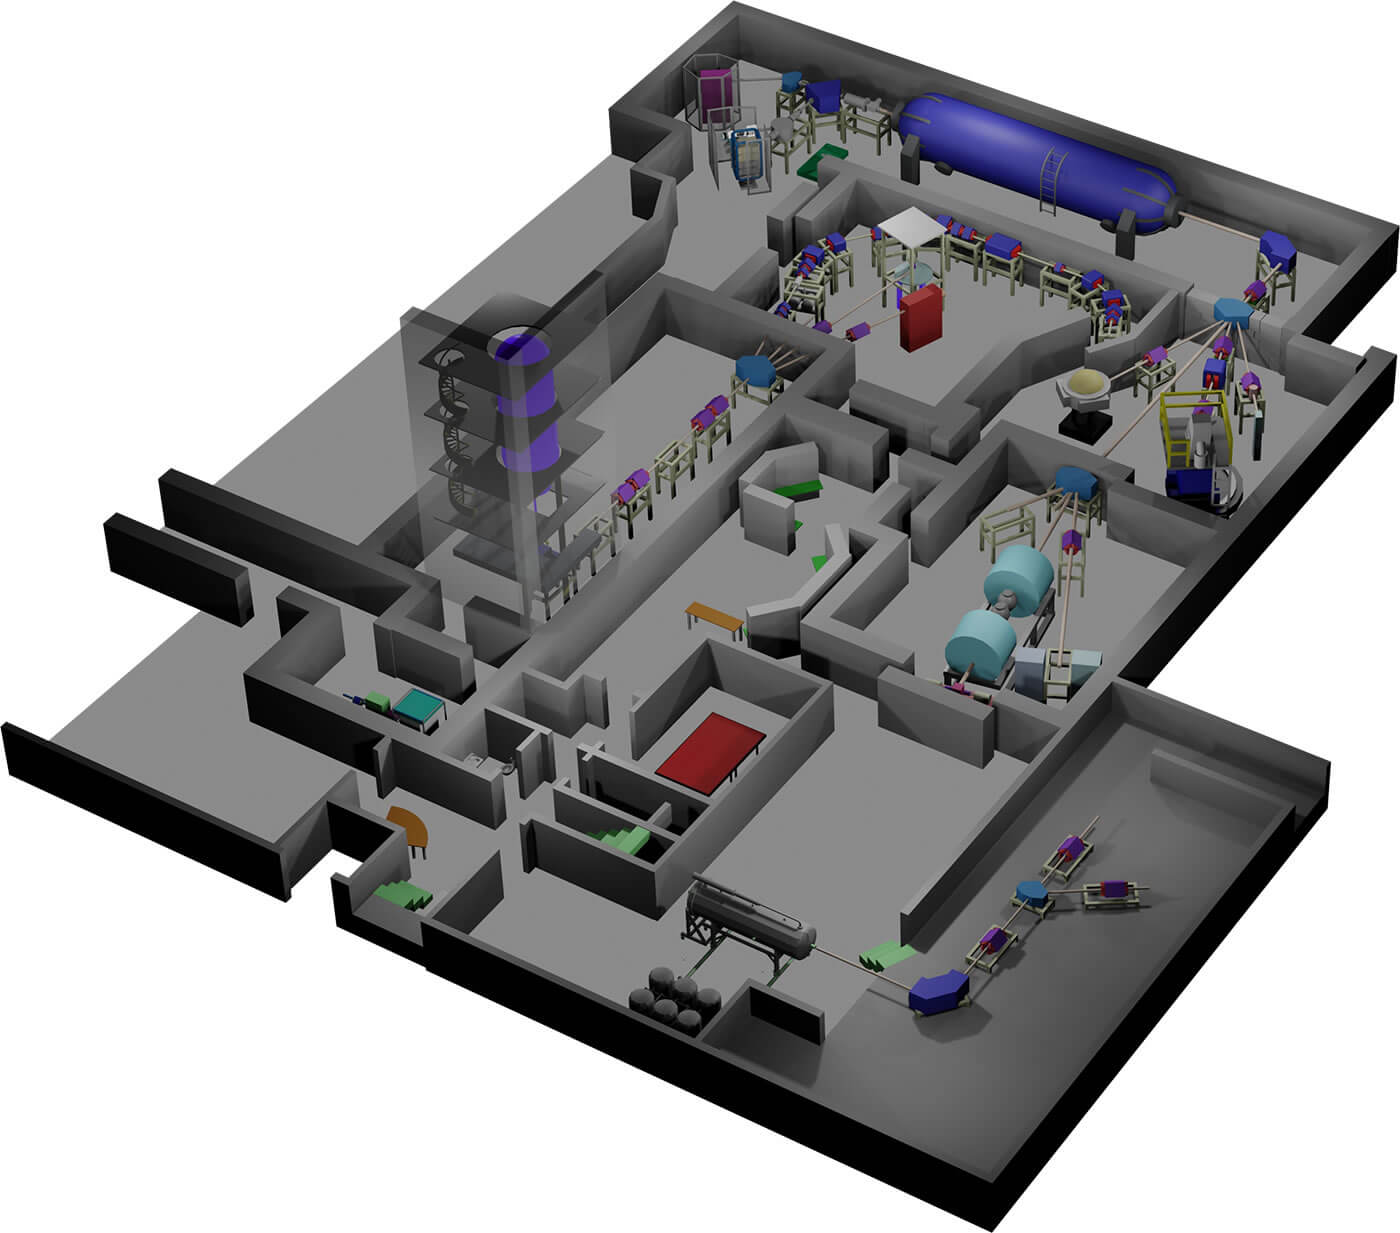
\includegraphics[scale=0.25]{Setup_Figs/NSL_2018_Layout.png}
    \caption{Current layout of the Nuclear Science Laboratory at Notre Dame.}
    \label{fig:NSL}
\end{figure}

The 10 MV FN Tandem has been in operation since 1968. It operates using a Van de Graaff system. Belts carrying a static charge deposit the charge on a terminal in the center of the machine. The charging belts are a pelletron system, upgraded from the original insulated belt system in 2000. The beamline is kept at vacuum, but the area outside of the beamline, but within the accelerator tank, is filled with a mixture of CO$_2$ and dry nitrogen gas, at approximately 200 PSI.

To create a more uniform acceleration field, the terminal is brought to ground along the beamline using resistor-lined tubes. The resistors used create a uniform electrical field down the tube, allowing for uniform acceleration.

It is known as a tandem because the system is a two-stage acceleration. Negatively charged ions enter the system, accelerating toward a positively charged terminal shell. Inside of the shell, the ions go through carbon stripping foils 12 $\mu g/cm^2$ thick, becoming positively charged as electrons are pulled off. The ions then accelerate away from the terminal for the second stage.

\begin{figure}
    \centering
    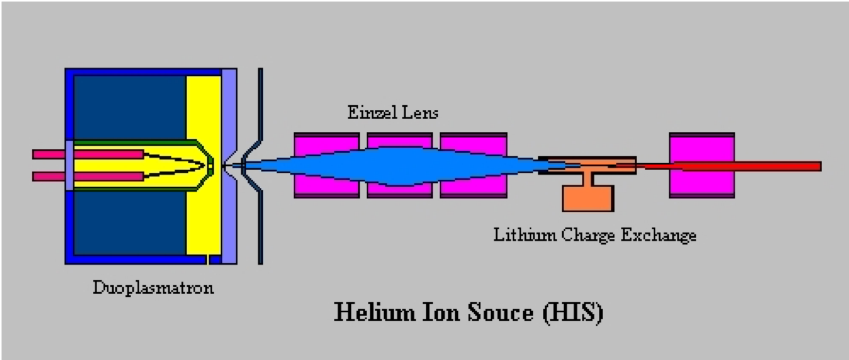
\includegraphics[scale=0.5]{Setup_Figs/HIS.png}
    \caption{A schematic of how the Helium Ion Source works.}
    \label{fig:HIS}
\end{figure}

\section{Target Fabrication}

For conversion electron experiments, thinner targets are ideal. Electrons must escape the target, and a thicker target causes energy loss and straggling effects, blurring out the conversion electron spectrum.

Enriched, self-supporting samarium targets were used for this experiment. The material started as Sm$_2$O$_3$. Using the reaction

\begin{equation}
    SmO_2 + Hf \xrightarrow{} HfO_2 + Sm
    \label{eq:sm_hf}
\end{equation}

at a temperature of [CHECK] the samarium was extracted as a metal. Once cooled, it was rolled as thin as possible. Samarium easily oxidizes, stagnating the rolling process, as too much work on the material at once could cause instantaneous oxidization, resulting in the loss of the target. Rolling had to be done incrementally, giving the material time to rest.

\section{Internal Conversion Electron Ball Spectrometer}

The Internal Conversion Electron Ball Spectrometer (ICEBall) was developed at the University of Pittsburgh by Metlay et al. \citep{metlay92:_iceball_comm,metlay93:_iceball_comm}. Originally at the Spin Spectrometer [CITE] at Oak Ridge National Laboratory, it was later stationed at the Wright Nuclear Structure Laboratory at Yale University with the YRAST Ball [CITE], until being brought to the University of Notre Dame and stationed in the Nuclear Science Laboratory West Target Room, on a dedicated beamline \citep{battaglia15:_iceball_176lu}.

Originally designed to go inside of large gamma detector arrays, ICEBall consists of six mini-orange spectrometers, cooled using liquid nitrogen to reduce background. 

\subsection{Detectors}

The detectors inside of ICEBall are lithium-drifted silicon detectors, known as Si(Li) detectors for short. Si(Li) detectors allow for a larger depletion region in the detector, compared to pure silicon detectors, and can be made thicker as a result. The detectors inside of ICEBall are 5mm thick, with a surface area of 750 mm$^2$ \citep{metlay93:_iceball_comm}.

Between the detectors and the target are mini-orange filter. Designed in the 1970s, mini-orange filters are a permanent magnet array surrounding a high-Z material, as seen in Figure \ref{fig:mini_orange}. In ICEBall, this material is tantalum [CHECK], and the magnets are made of SmCo$_5$, and arranged in groups of 3. The tantalum acts as a blocker, lowering noise from the target that can be due to $\gamma$ or $\delta$ rays. The magnets create a field that bends electrons toward the detector, while bending positrons away from the detector, further lowering noise. 

\begin{figure}
    \centering
    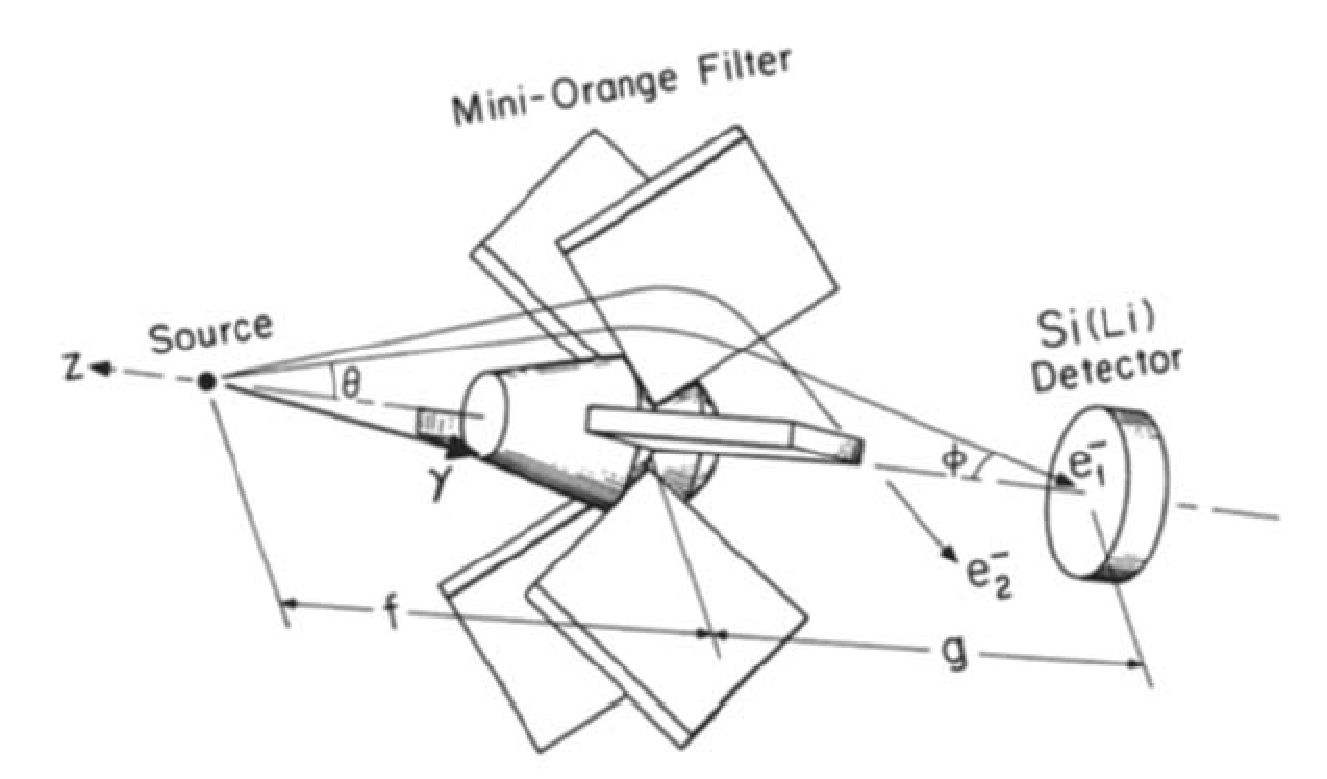
\includegraphics[scale=0.6]{Setup_Figs/mini-orange-metlay-figure.pdf}
    \caption{Graphic of the mini-orange filter. The central blocker keeps $\gamma$-rays from hitting the detector. The magnets bend electrons toward the detectors, and positrons away from the detectors. Being permanent magnets, they are optimized for a range of electron energies, and can cause overbending or underbending of electrons outside of that energy range, making the magnetic filter a factor in the efficiency. Taken from \citep{metlay93:_iceball_comm}}
    \label{fig:mini_orange}
\end{figure}

A large drawback of these mini-orange filters is the permanent magnets. The field is optimized for a range of energies, and must be pre-selected before the experiment. Switching magnets mid-experiment is not feasible, due to the downtime needed to warm-up the system, bring it to atmosphere, replace the filter, and then reverse the first two steps. Additionally, the mini-orange filter changes the efficiency of the system, meaning each configuration must have a separate efficiency measurement.

\begin{table}[]
    \centering
    \caption{ICEBall magnetic strengths with GEORGINA}
    \begin{tabular}{c|c|c} \toprule
         Detector & Filter & Strengths \\
         \hline
         1 & M13 & 815,740,830 \\ 
         2 & M15 & 939,911,949\\
         3 & M21 & 850,875,900 \\
         4 & M14 & 972,911,992\\
         5 & M18 & 856,913,963\\
         6 & M22 & 845,900,900\\ \bottomrule
    \end{tabular}
    \footnotesize
    \item Magnetic strengths of the mini-orange filters used in the GEORGINA experiments, listed in Gauss. 
    \label{tab:ICE_Magnet}
\end{table}

\begin{table}[]
    \centering
    \caption{ICEBall magnetic strengths with Clovershare}
    \begin{tabular}{c|c|c} \toprule
         Detector & Filter & Strengths \\
         \hline
         1 & M13 & 815,740,830 \\ 
         2 & M20 & 1228,1292,1265\\
         3 & M21 & 850,875,900 \\
         4 & M2 & 31411,1420,1410\\
         5 & M16 & 1286,1340,1285\\
         6 & M22 & 845,900,900\\ \bottomrule
    \end{tabular}
    \footnotesize
    \item Magnetic strengths of the mini-orange filters used in the Clovershare experiments, listed in Gauss. 
    \label{tab:ICE_Magnet}
\end{table}

\begin{table}[]
    \centering
    \caption{ICEBall detector locations }
    \begin{tabular}{c|c|c} \toprule
         Detector & $\theta$ & $\phi$  \\
         \hline
         1 & 90 & 79.2 \\ 
         2 & 270 & 100.8\\
         3 & 172 & 129.9\\
         4 & 198 & 31.7\\
         5 & 18 & 148.3\\
         6 & 355 & 50.1\\ \bottomrule
    \end{tabular}
    \footnotesize
    \item The beam axis is the z-axis. $\theta$ is the angle in the xy-plane, where 0 degrees is beam left. $\phi$ is the azimuthal angle, with respect to the beam axis. All values are in degrees.
    \label{tab:ICE_Det_Loc}
\end{table}

\subsection{Calibration}

ICEBall is calibrated using two sources: $^{133}$Ba and $^{207}$Bi. The specific properties of the two sources are listed in Table \ref{Table:Sources}. The $^{207}$Bi covered the high-energy regime, with lines around 500 keV and 1000 keV. The $^{133}$Ba covered energies from 200 to 400 keV. Both sources are low activity, preventing incomplete or overlapping charge collection from hindering the resolution of the detectors during calibration runs.

\begin{table}[]
    \centering
    \caption{ICEBall calibration sources}
    \begin{tabular}{c|c|c|c|c} \toprule
         Source & Activity & Date Measured & Energy (keV) & Intensity (\%)\\
          \hline 
         $^{133}$Ba & May-4-2012 & 0.331(7) $\mu$C & 240.413 & 0.331 \\
         & & & 266.868 & 0.698 \\
         & & & 320.032 & 1.308 \\
         & & & 347.866 & 0.370 \\
         \hline
         $^{207}$Bi & May-4-2012 & 0.306(8) $\mu$C & 481.697 & 1.562 \\ 
         & & & 554.4 & 0.469 \\
         & & & 975.657 & 7.243 \\
         & & & 1048.1 & 1.838 \\\bottomrule
    \end{tabular}
    \footnotesize
    \item Calibration source information for ICEBall. The energies and the respective intensities are listed for each source. Intensities are taken from \cite{trzaska90:_calibration}. The intensity of the 347 keV line in $^{133}$Ba is both the 384K and 356L intensities combined.
    \label{tab:ICE_Cal_Source}
\end{table}

The energy calibration is assumed to be quadratic in nature, although both linear and quadratic calibrations are performed. [FIGURE]

The efficiency calibration is fitted to equation

\begin{equation}
    ln(\epsilon) = p_1+p_2ln(E)+p_3E
    \label{eq:SiLi_Eff}
\end{equation}

The efficiency is a convolution of the magnetic configuration and the inherent detector efficiency. Using the efficiency points, the analytic expression for the efficiency was determined empirically in previous work \citep{battaglia15:_iceball_176lu}.

\section{GEORGINA}

GEORGINA is a compact array of germanium detectors for $\gamma$-ray experiments. The detectors are 100\% relative efficiency. These detectors were designed for use with astrophysical capture reactions, meant to cover a large solid angle. There are a total of five detectors.

\subsection{Detectors}

While the GEORGINA detectors were designed for reasonable efficiency up to 12 MeV, they were used in this experiment to look at energies up to 4 MeV. Two detectors of the five were used in this experiment. 

The detectors were designed with the crystal at a $90^{\circ}$ from the cold-finger, as seen in Figure \ref{fig:georgina}.

\begin{figure}
    \centering
    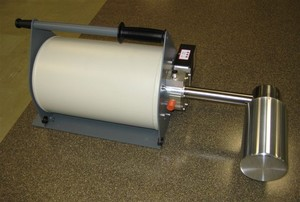
\includegraphics{Setup_Figs/georgina_example.png}
    \caption{An example of one of the GEORGINA detectors. The crystal is at a $90^{\circ}$ from the cold finger, allowing the long side of the crystal to be placed next to the target, to optimize solid angle coverage. In the experiment, the circular face of the crystal was placed toward the target.}
    \label{fig:georgina}
\end{figure}

\begin{table}[]
    \centering
    \caption{GEORGINA detector locations }
    \begin{tabular}{c|c|c} \toprule
         Detector & $\theta$ & $\phi$  \\
         \hline
         1 & 0 & 90 \\ 
         2 & 180 & 90\\ \bottomrule
    \end{tabular}
    \footnotesize
    \item The beam axis is the z-axis. $\theta$ is the angle in the xy-plane, where 0 degrees is beam left. $\phi$ is the azimuthal angle, with respect to the beam axis. All values are in degrees.
    \label{tab:GEORGE_Det_Loc}
\end{table}

\subsection{Calibration}

The GEORGINA detectors were calibrated using a $^{152}$Eu source, in addition to the ICEBall sources. The information about the sources is in Table \ref{tab:GEORGINA_Cal_Source}. Additionally, several background lines could be used to extend the energy calibration up to 2700 keV. 

\begin{table}[]
    \centering
    \caption{GEORGINA calibration sources}
    \begin{tabular}{c|c|c|c|c} \toprule
         Source & Activity & Date Measured & Energy (keV) & Intensity (\%)\\
          \hline 
         $^{133}$Ba & May-4-2012 & 0.331(7) $\mu$C & 80.997 & 0.3406 \\
         & & & 276.398 & 7.164 \\
         & & & 302.853 & 18.33 \\
         & & & 356.017 & 62.05 \\
         & & & 383.851 & 8.94 \\
         \hline
         $^{207}$Bi & May-4-2012 & 0.306(8) $\mu$C & 569.702 & 97.75 \\ 
         & & & 1063.662 & 74.09 \\
         \hline
         $^{152}$Eu & & & 121.7825 & 28.65 \\
         & & & 244.6989 & 7.582 \\
         & & & 344.281 & 26.6 \\
         & & & 411.115 & 2.262 \\
         & & & 443.965 & 3.125 \\
         & & & 778.903 & 13.017 \\
         & & & 867.39 & 4.26 \\
         & & & 964.055 & 14.758 \\
         & & & 1085.842 & 10.062 \\
         & & & 1089.7 & 1.738 \\
         & & & 1112.087 & 13.587 \\
         & & & 1408.022 & 20.945 \\\bottomrule
    \end{tabular}
    \footnotesize
    \item Calibration source information for GEORGINA. The energies and the respective intensities are listed for each source. Intensities are taken from \cite{trzaska90:_calibration}. The  $^{152}$Eu does not have activity and intensity, as it was normalized to the $^{133}$Ba.
    \label{tab:GEORGINA_Cal_Source}
\end{table}

The efficiency calibration is fitted to equation

\begin{equation}
    ln(\epsilon) = a_0-(a_1+a_2\times e^{-a_3\times E})\times E^{-a_4\times E}\times ln(E)
    \label{eq:Ge_Eff}
\end{equation}

\subsection{Electronics}

% we need shit from Tony's thesis for this dawg

\section{CloverShare}

CloverShare is a group of HPGe clover detectors with BGO shields, that originated at Yale University. They were sent to various laboratories and universities for series of experiments, including the NSL. Two campaigns of experiments were run with CloverShare, each one involving an ICEBall experiment.

\subsection{Detectors}

The CloverShare detectors are large, segmented HPGe detectors, with fitted BGO shields. In the first of the two experiments, 7 detectors were used. In the second, 5 were used, as two experienced pre-amplifier problems during the previous campaign. The detectors used biases between -3000 and -4000 V, and were kept cold using a liquid nitrogen autofill system.

Due to the fixed nature of the ICEBall detectors, the clovers were limited in the angles they could be placed at, to optimize efficiency. With the tantalum blockers in front of the Si(Li) detectors to block gamma-rays and x-rays, placing the clovers behind these detectors would drastically reduce efficiency.

\subsection{Calibration}

The CloverShare detectors were calibrated using the same sources as GEORGINA, as well as at $^{56}$Co source that was created on the FN accelerator days before the experiment. The information about the sources is in Table \ref{tab:GEORGINA_Cal_Source} and \ref{tab:Co_Energy}. 

\begin{table}[]
    \centering
    \caption{$^56$Co calibration information}
    \begin{tabular}{c|c|c|c}
         Activity & Date Measured & Energies  \hline \\
         6.44 $\mu$Ci & Mar-16-2016 & 846.77 \\
         & & 977.372 \\
         & & 1037.843 \\
         & & 1175.101 \\
         & & 1238.288 \\
         & & 1360.212 \\
         & & 1771.357 \\
         & & 2015.215 \\
         & & 2034.791 \\
         & & 2598.5 \\
    \end{tabular}
    \caption{Energies used in $^{56}$Co for calibration, as well as activity.}
    \label{tab:Co_Energy}
\end{table}

The $^{152}$Eu was placed on the individual detectors instead of centered in the trap, as it was not mounting well to the target ladder. To use the $^{152}$Eu for efficiency, a linear extrapolation of the efficiency of the 344 keV line was done using the 303 keV and 356 keV lines in $^{133}$Ba. All points in the Eu were then scaled based on this. A characteristic fit of the efficiency of these detectors can be seen in Figure \ref{fig:Clover_eff}, with the various sources denoted for the points.

\begin{figure}
    \centering
    \includegraphics{}
    \caption{Efficiency of CloverShare detector [INSERT]. The different colors/shapes indicate the different sources, as labeled. The fit is also included.}
    \label{fig:Clover_eff}
\end{figure}

As the clovers are comprised of four separate crystals, the efficiency was taken for the individual leaves, and once the detectors had been calibrated, they were summed together. Figure \ref{fig:Clover_ind_vs_sum} shows the comparison. As is expected, there is a small improvement in the higher energies. The summed crystals were used for analysis, and will be used in spectra from here on forward.

\begin{figure}
    \centering
    \includegraphics{}
    \caption{Efficiency of CloverShare detector [INSERT], with the individual leaves' efficiency summed together, compared to the efficiency of the leaves calibrated and summed together. The different colors/shapes indicate the different sources, as labeled. The fit is also included.}
    \label{fig:Clover_ind_vs_sum}
\end{figure}

% Uggghhhhh, fuck this shit. Stuff of nightmares.

Each leaf of the clovers was energy calibrated. An unusual trend in the residuals was found in all cases, as seen in \ref{fig:Clover_ene_res}. This trend could not be corrected for by using a higher-order polynomial, as is usually the case for integral non-linearities in multi-channel analyzers \citep{knoll00:rad_det_meas}. Instead, this appears to be a differential non-linearity in the electronics, resulting in discontinuities. As will be discussed in the next section, the electronics used for the experiment are not used with detectors of this sensitivity.

\subsection{Electronics}

% gotta talk to Anna about those HECTOR electronics

\section{Determination of Running Energy}

Because of the use of HPGe detectors in an $(\alpha,2n)$ reaction, the neutron flux must be minimized in comparison to the cross section of the reaction, as the $(\alpha,n)$ reaction is also open. To do this, a range of energies to test were selected by looking at theoretical cross sections in Talys. These energies were then tested with natural Sm targets, ICEBall, and two liquid scintillators to detect neutrons.

Samarium, as with many even-Z elements in the lanthanide region, has many stable isotopes. A total of five stable isotopes of Samarium exist, with two other isotopes being long-lived. Table \ref{tab:nat_Sm} summarizes the abundances and lifetimes of the various isotopes found in natural Samarium. The two isotopes to be used in enriched targets in the experiments have the highest natural abundances, $^{152,154}$Sm.

\begin{table}[]
    \centering
    \begin{tabular}{c|c|c}
    \toprule
         Isotope & Lifetime (y) & Abundance (\%)  \\
         \hline
         $^{144}$Sm & Stable & 3.08 \\
         $^{147}$Sm & $1.06\times10^{11}$ & 15.00 \\
         $^{148}$Sm & $7\times10^{15}$ & 11.25 \\
         $^{149}$Sm & Stable & 13.82 \\
         $^{150}$Sm & Stable & 7.37 \\
         $^{152}$Sm & Stable & 26.74 \\
         $^{154}$Sm & Stable & 22.74 \\
         \bottomrule
    \end{tabular}
    \caption{Isotope Distribution of Natural Samarium}
    \label{tab:nat_Sm}
\end{table}

\subsection{Talys Calculations}

Talys \citep{koning07:_talys} is software for the simulation of nuclear reactions. Cross sections can be estimated using Talys to guide where an experiment may want to run to optimize production, as is the case presently. 

\subsection{Test Analysis and Results}

Once the detectors were calibrated, each energy was run, with a total of four different targets across six energies. For each energy, the peaks in the electron spectra were identified with their respective isotopes, working under the assumption that only the lowest-lying states and the ground-state band would be populated significantly enough to see the electrons. The K-electron of the $4^+\rightarrow2^+$ ground state transition for both nuclei of interest was clearly visible and clean at all energies. These K-electrons were used for the cross-section calculation.

To calculate the cross section, the formula

\begin{equation}
    \sigma=\frac{Yield}{\delta x*Q*\epsilon}
    \label{eq:xs}
\end{equation}

was used, where $\delta x$ is the target thickness, $Q$ is the integrated charge, and $\epsilon$ is the efficiency of the Si(Li) detector at the electron energy. The $Yield$ is the area under the curve.

This then had to be compared with the neutron flux. A bunched beam was used to get a time-of-flight. Calculating the neutron flux was done using the formula

\begin{equation}
    Flux = \frac{Neutrons}{\delta x*Q}
\end{equation}

where $\delta x$ and $Q$ are the same as used for the cross section. The neutron yield is obtained by looking at the liquid scintillator energy vs time-of-flight, as seen in Figure \ref{fig:neutron}. The left-most line is the gamma-flash that comes from the prompt gammas. The secondary gathering of counts, to the right, is the neutron peak. This area can be integrated over to get the number of neutrons seen during the run.

Table \ref{tab:neutrons} summarizes the results at each energy. Note, that the cross section is not reflective of the full cross section of the isotopes, but of the K-electrons for that transition. The rightmost column is also shown in Figure \ref{fig:xs_neutron}. This ratio, of the cross-section to the neutron flux, was ultimately used to determine the running energy. The two higher energies, 20 and 21 MeV, have a ratio that agrees within error for both isotopes. Ultimately, 20 MeV was chosen for two reasons: to minimize any higher energy reaction channels, and because the neutron flux was lower in rate.

\begin{table}[]
    \centering
    \begin{tabular}{c|c|c|c|c|c}
        \toprule
        & \multicolumn{2}{c|}{Cross Section (mb)} & Neutron Flux & \multicolumn{2}{c}{Ratio ($\sigma/\Phi_n$)} \\
        Energy (MeV) & $^{154}$Gd & $^{154}$Gd & (neutrons/s) & $^{154}$Gd & $^{154}$Gd \\
        \hline
        16 & 0.126 (13) & 0.334 (25) & 1.247 (4) & 0.101 (10) & 0.268 (20)\\
        17 & 0.554 (54) & 1.273 (91) & 2.142 (13) & 0.259 (25) & 0.594 (43)\\
        18 & 3.124 (133) & 5.427 (233) & 4.281 (30) & 0.730 (31) & 1.268 (55)\\
        19 & 3.030 (172) & 5.327 (217) & 4.205 (25) & 0.721 (41) & 1.267 (52)\\
        20 & 5.618 (167) & 9.438 (275) & 5.806 (36) & 0.968 (29) & 1.626 (48)\\
        21 & 7.438 (267) & 12.827 (419) & 7.410 (54) & 1.004 (37) & 1.731 (58)\\ 
        \bottomrule
    \end{tabular}
    \caption{Summary of Energy Tests}
    \label{tab:neutrons}
\end{table}

% % uncomment the following lines,
% if using chapter-wise bibliography
%
% \bibliographystyle{ndnatbib}
% \bibliography{example}
